
\documentclass[11pt]{beamer}
\usepackage[utf8]{inputenc}
\usepackage[T1]{fontenc}
\usepackage[portuguese]{babel}
\usepackage{amsmath}
\usepackage{amsfonts}
\usepackage{amssymb}
\usepackage{graphicx, tabularx, multirow, multicol}
\usepackage{caption}
\usepackage{svg}
\usepackage{booktabs} % For prettier tables [new]
\usepackage{ragged2e} % justifying [new]


\usetheme{Berlin}
\usecolortheme{beaver}

\makeatletter
\newlength\beamerleftmargin
\setlength\beamerleftmargin{\Gm@lmargin}
\makeatother


\newcommand{\backupbegin}{
   \newcounter{framenumberappendix}
   \setcounter{framenumberappendix}{\value{framenumber}}
}
\newcommand{\backupend}{
   \addtocounter{framenumberappendix}{-\value{framenumber}}
   \addtocounter{framenumber}{\value{framenumberappendix}}
}

\usepackage[style=abnt]{biblatex}
\addbibresource{./refs.bib}


	\author{Gabriel Petrini}
	\title{Três Ensaios em Macroeconomia Imobiliária}
	\subtitle{Instituições, Inflação de Ativos e Instabilidade Financeira}
	\institute{IE/Unicamp}
	\date{01 de Junho de 2021}
    \setbeamercovered{transparent}
	\setbeamertemplate{navigation symbols}{}
	\apptocmd{\frame}{}{\justifying}{} % Allow optional arguments after frame.

\AtBeginSection[]
{
    \begin{frame}
        \frametitle{Ensaios}
        \tableofcontents[currentsection]
    \end{frame}
}
\begin{document}

\begin{frame}[plain]
	\maketitle
\end{frame}

\section[Introdução]{Introdução e Justificativa}

\begin{frame}{Hein?! Macroeconomia Imobiliária?}

A literatura macroeconômica tem abordado os seguintes temas separadamente:

\begin{itemize}
    \item mudanças na composição patrimonial dos bancos comerciais;
    \item papel do investimento residencial e de bolhas de ativos na dinâmica macroeconômica;
    \item endividamento, crise e fragilidade financeira das famílias.
\end{itemize}

\begin{alert}{Macroeconomia Imobiliária}

Esforço de conectar o lado real e financeiro da economia relacionando os impactos, as mudanças e as consequências macroeconômicas do mercado imobiliário.

Os ensaios exploram as diferentes dimensões da macroeconomia imobiliária
\end{alert}

\end{frame}

\begin{frame}{Hipotecarização}
\framesubtitle{Ah tá, financeirização dos imóveis? NÃO!}

\begin{figure}[H]
	\centering
	\caption{Participação do empréstimo imobiliário no total do balanço patrimonial dos bancos (1870-2016)}
	\label{GraficoJorda}
	\includegraphics[width=.75\paperwidth, height=.43\paperheight]{../../Writings/QCA/plots/Jorda_Facet.png}
	\caption*{\textbf{Fonte:} \textcite{jorda_rate_2019}}
\end{figure}

\end{frame}

\section[QCA]{\textbf{Ensaio 1:} Características institucionais}

\begin{frame}{Literatura e suas Lacunas}
\framesubtitle{Análises institucionais comparadas}

\begin{description}
    \item[CPE:] Conceituam o papel macroeconômico do setor financeiro
        \begin{description}
            \item[VoC:] questões microeconômicas e relacionadas à oferta de crédito
        \end{description}
    \item[Financeirização:] pouca atenção às famílias e ao investimento residencial
\end{description}

\begin{alert}{Lacunas em comum}

Pouca ênfase às institucionalidades do mercado imobiliário; à composição e aos determinantes
do crescimento do setor financeiro.

\textbf{Estudos de caso:} amostras pequenas (max. 4).

\textbf{Análise Quantitativa:} Instituições $\to$ efeitos marg. (simétricos).

\end{alert}

\end{frame}


\begin{frame}{Objetivo e Metodologia}

\begin{description}
    \item[Objetivo:]  examinar as configurações institucionais que determinam o grau de hipotecarização do sistema bancário de um país
    \item[Hipótese:] institucionalidade presente nos diversos sistemas financeiros é relevante para explicar o grau de hipotecarização
        \begin{itemize}
            \item ausência de uniformidade causal do arranjo institucional \cite{chang_institutions_2011}
        \end{itemize}
    \item[Metodologia:] \textit{fuzzy-set} QCA (fsQCA)
    \item[Recorte:] Países da base de dados de \textcite{jorda_rate_2019} para os anos de 1980 a 2016
\end{description}
\end{frame}

\section[Painel]{\textbf{Ensaio 2:} Investimento residencial e a dinâmica macroeconômica}

\begin{frame}{Objetivo e Metodologia}

\begin{description}
    \item[Objetivo:]  Estimar os determinantes do investimento residencial

        \begin{itemize}
            \item Investigar a capacidade explicativa da Tx. Própria para outros países
        \end{itemize}

    \item[Hipótese:] Investimento residencial depende tanto da concessão de crédito quanto da bolha de ativos
    \item[Metodologia:] Modelo de Séries Temporais em Painel
    \item[Recorte:] Países da base de dados de \textcite{jorda_rate_2019} para os anos de 1980 a 2016
\end{description}
\end{frame}

\section[AB-SFC]{\textbf{Ensaio 3:} Dimensão real e financeira do mercado imobiliário}

\begin{frame}{Nova Narrativa}
\framesubtitle{Participação na execução hipotecária a partir da avaliação de risco}


\begin{figure}
    \centering
    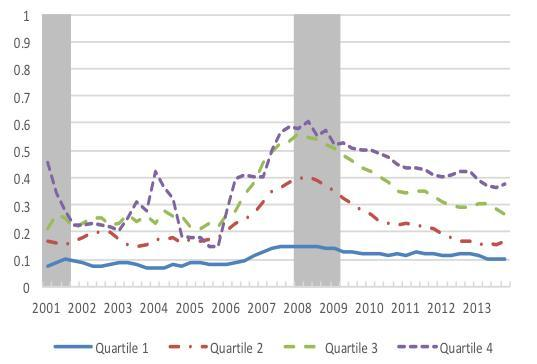
\includegraphics[width=.8\paperwidth, height=.6\paperheight]{figs/NovaNarrativa.png}
\end{figure}

\end{frame}



\begin{frame}{Objetivo e Metodologia}

\begin{description}
    \item[Objetivo:]  avaliar as implicações macroeconômicas de um sistema bancário ativo com ciclo de crédito endógeno
\item[Hipótese:] somente as famílias com melhor avaliação de risco investem em imóveis e ampliam a demanda por crédito na medida que seu colateral com os bancos se valoriza $\sim$ Nova Narrativa
    \item[Metodologia:] modelo AB-SFC de simulação com famílias heterogêneas e investimento residencial explicitamente modelado
\end{description}
\end{frame}

\begin{frame}{Estrutura do modelo}

\begin{figure}
    \centering
    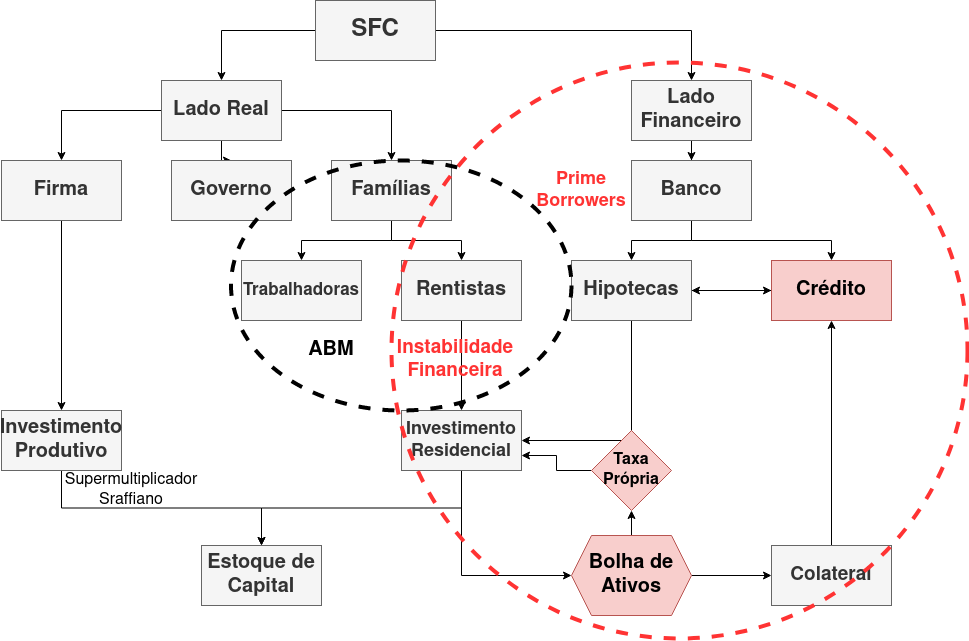
\includegraphics[width=.8\paperwidth, height=.67\paperheight]{./figs/Diagrama_ABSFC.png}
\end{figure}

\end{frame}


\section{Contribuições}

\begin{frame}{Contribuições esperadas}

\textbf{QCA:} configurações institucionais $\to$ hipotecarização
\\~\\
\textbf{Painel:} estimar os determinantes do investimento residencial
\\~\\
\textbf{AB-SFC:} explicitar o papel da inflação de ativos na instabilidade financeira das famílias

\end{frame}

\begin{frame}[allowframebreaks]{Referências}
\printbibliography
\end{frame}



\appendix
\backupbegin

\begin{frame}{Características institucionais de alguns países da OCDE}
\framesubtitle{Dimensão qualitativa da Macroeconomia Imobiliária}
    \begin{table}[htb]
	\centering
	\caption{Características institucionais de alguns países europeus da OCDE}
	\label{Institucional}
		\resizebox{.7\textwidth}{!}{%
			\begin{tabular}{c|c|c|c|c|c|c}
				\hline\hline \\
				\multirow{2}{*}{\textbf{Países}} & \multicolumn{6}{c}{\textbf{Características institucionais}} \\\cline{2-7}
				&
				\textbf{\begin{tabular}[c]{@{}c@{}}Maturidade\\ Hipotecária\\(meses)\end{tabular}} &
				\textbf{\begin{tabular}[c]{@{}c@{}}Taxa de juros\\ Hipotecária\end{tabular}} &
				\textbf{\begin{tabular}[c]{@{}c@{}}Reembolso antecipado:\\ Contratado (C)/\\ Legislado (L)\end{tabular}} &
				\textbf{\begin{tabular}[c]{@{}c@{}}Possibilidade de segunda\\hipoteca a partir\\da valorização do imóvel\end{tabular}} &
				\textbf{\begin{tabular}[c]{@{}c@{}}Financiamento pelo\\ Mercado de capitais (\%)\end{tabular}} &
				\textbf{\begin{tabular}[c]{@{}c@{}}Execução\\ Hipotecária\\(meses)\end{tabular}} \\\hline
				\textbf{Alemanha}                & 30   & Fixa       & C/L   & Não permitido    & 14   & 9    \\\hline
				\textbf{Espanha}                 & 30   & Variável   & C/L   & Limitado         & 45   & 8    \\\hline
				\textbf{França}                  & 19   & Fixa       & C/L   & Não permitido    & 12   & 20   \\\hline
				\textbf{Holanda}                 & 30   & Fixa       & C     & Permitido        & 25   & 5    \\\hline
				\textbf{Itália}                  & 22   & Variável   & L     & Não permitido    & 20   & 56   \\\hline
				\textbf{Portugal}                & 40   & Variável   & L     & Sem informação   & 27   & 24  \\\hline
				\hline
				
			\end{tabular}%
		}
	\caption*{\textbf{Fonte:}  \textcite[p.~94, adaptado e traduzido]{van_gunten_varieties_2018}}
\end{table}
\end{frame}

\begin{frame}{O que diabos é QCA?}
\framesubtitle{(Mas e o \textit{probit}?)}

\textbf{QCA:} Qualitative Comparative Analysis

 Desenvolvida originalmente por \textcite{ragin_comparative_1989}, esta metodologia associa todas as configurações possíveis das variáveis explicativas a um resultado específico por meio de operações lógicas e teoria dos conjuntos.

Permite identificar as condições necessárias e suficientes para ocorrência da hipotecarização

\begin{itemize}
    \item Equifinalidade
    \item Causação conjuntural
    \item Causação assimétrica
\end{itemize}
\end{frame}
\backupend
\end{document}
